\begin{frame}[hasprev=false,hasnext=true]
\label{example:identifier-def-clear-path}
\frametitle{Definition-clear paths example}

Consider the following graph:

\begin{figure}
	\centering
	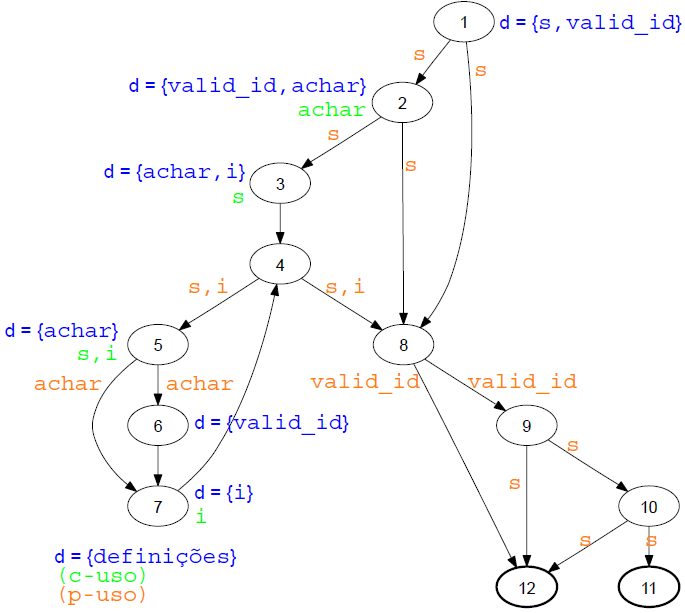
\includegraphics[scale=.3]{aux/examples/identifier-def-clear-path/identifier-java-dug}
\end{figure}

\end{frame}



\begin{frame}[hasprev=true,hasnext=false]
\frametitle{Definition-clear paths example}

\begin{itemize}
	\item Path (1,8,12) is a definition-clear path with respect to
	\srccode{valid_id} defined at node 1.

	\item Path (1,2,8,12) is not a definition-clear path with respect to
	\srccode{valid_id} defined at node 1, because \srccode{valid_id} is
	redefined at node 2.
\end{itemize}

\end{frame}